
\medskip
A figura 5 mostra o modelo lógico do sistema, no qual pode-se observar que as tabelas seguem a 
lógica proposta no diagrama DER. A base do sistema reside na gestão de contas: cada \textbf{usuário} 
pode gerenciar múltiplas 
\textbf{propriedades}, mas cada propriedade é estritamente vinculada a um único usuário. Esta relação 
de um para muitos é o ponto de partida para toda a organização dos dados no sistema.

\medskip
Em seguida, o foco se move para a estrutura física. Uma única \textbf{propriedade} é subdividida 
em múltiplos \textbf{talhões}, que são as áreas de monitoramento. Cada talhão, por sua vez, pertence 
exclusivamente àquela propriedade, estabelecendo uma clara hierarquia de localização dentro do sistema.

\medskip
O \textbf{talhão} é o elo que conecta a área de terra ao monitoramento. Ele agrupa os \textbf{pés} 
(plantas individuais) sob sua área, e é o registro obrigatório para os \textbf{históricos} de 
monitoramento, garantindo que qualquer medição seja sempre associada a uma área específica.

\medskip
Os \textbf{pés} de plantas são o núcleo da avaliação. É neles que se coletam \textbf{fotos} como
evidência visual e se elaboram os \textbf{relatórios} de diagnóstico. O pé também pode receber um 
registro de \textbf{histórico} específico, embora este seja opcional em comparação ao registro de 
histórico do talhão.

\medskip
Finalmente, os \textbf{relatórios} servem como o documento final de análise. Eles consolidam a 
avaliação de um \textbf{pé} específico e incluem as \textbf{fotos} coletadas como parte da documentação. 
Embora um relatório possa ter múltiplas fotos, cada foto usada no processo é estritamente ligada a um 
único relatório de análise.

\medskip
\begin{figure}[H]
\centering
\caption{Diagrama Modelo Logico}
\label{fig:diagrama-mer}
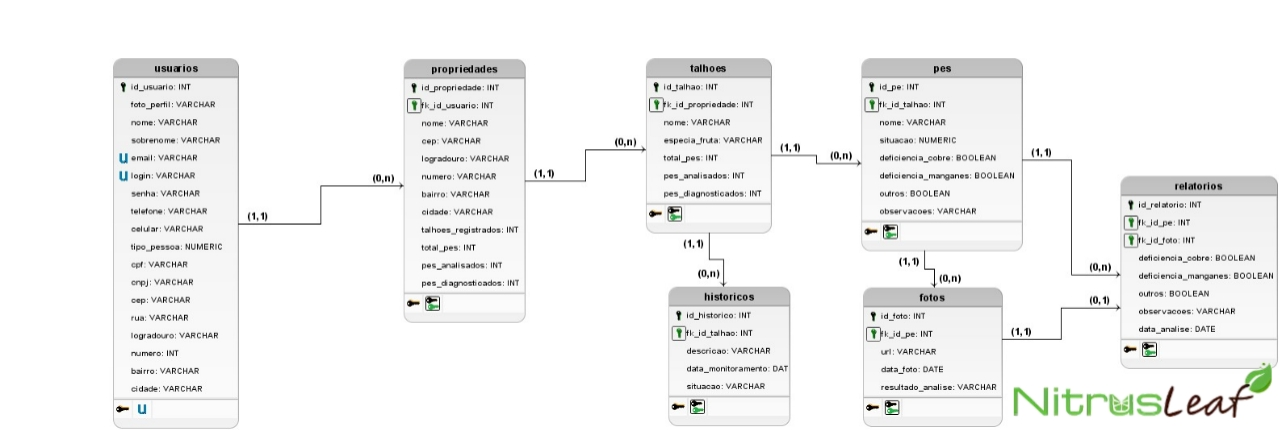
\includegraphics[width=0.9\textwidth]{Images/DiagramaMER.jpg}
\SourceOrNote{Equipe 21 - Vitalliz (2025)}
\end{figure}

Esse modelo é essencial para a posterior geração do modelo físico, que será
utilizado na criação e estruturação do banco de dados real.
\medskip